\documentclass[11pt]{article}

%%%%%%%%%%%%%%%%%%%%%%%%%%%%%%%%%%%%%%%%%%%%%%%%%%%%
% Preamble:
%%%%%%%%%%%%%%%%%%%%%%%%%%%%%%%%%%%%%%%%%%%%%%%%%%%%
% Typical Packages:
\usepackage[utf8]{inputenc}
\usepackage{fullpage}
\usepackage{amsfonts}
\usepackage{amsmath}
\usepackage{amsthm}
\usepackage{amssymb}
\usepackage{mathrsfs}
\usepackage{graphicx}
\usepackage{color}
\usepackage{palatino}
\usepackage{url}
\usepackage{multicol}
\usepackage{enumerate}
\usepackage{ulem}
\usepackage{tikz}
\usepackage{tipa} 
\usepackage{upgreek}
\usepackage{hyperref}
\usepackage{verbatim}
\usepackage{caption}
\usepackage{fancyhdr}

\thispagestyle{empty}

% Title
\title{An Example Latex Document}
\author{Brooks Emerick}
\date{\today}

%%%%%%%%%%%%%%%%%%%%%%%%%%%%%%%%%%%%%%%%%%%%%%%%%%%%
% Start Document:
%%%%%%%%%%%%%%%%%%%%%%%%%%%%%%%%%%%%%%%%%%%%%%%%%%%%
\begin{document}

\maketitle

% Section
\section{Section 1 Title}
Hi, my name is Brooks. You can use ``section'', ``subsection'', and ``subsubsection'' to separate your write-up into appropriate sections.  Notice how I'm typing quotations! 

\subsection{This is the title for subsection 1.1}

\subsubsection{This is the title for subsubsection 1.1.1}

If you wish to suppress the label of the section, you can put a ``*'' next to the word ``section'' like so:

\subsection*{This is the title for a subsection without a label}

This is how you make a bulleted list: 

\begin{itemize}
    \item Project 1 
    \item Project 2
    \item Project 3
\end{itemize}

This is how you make an enumerated list:
\begin{enumerate}
    \item Stuff 1
    \item Stuff 2
\end{enumerate}

This is how you make an enumerated list with your very own enumeration scheme: 
\begin{enumerate}
    \item[(1.)] Stuff 1
    \item[(2.)] Stuff 2
\end{enumerate}



% New Page:
\pagebreak


% Section
\section{Math Stuff}
The fundamental theorem of calculus part 2 is 
$$\int_{a}^{b} f(x) dx = F(b) - F(a) $$

\noindent Let $\alpha$ be any real number between $0$ and $1$.  Let $\beta = \frac{1}{2}$.  Notice how the fraction $\frac{1}{2}$ is the same size as the text that surrounds it.  If you want it to be bigger, do this $\displaystyle \frac{1}{2}$.  

Consider the following system of equations: 

\begin{align}
    \frac{dx}{dt} & = 3x + 2y \label{Eqn_1} \\ 
    \frac{dy}{dt} & = 2x - 3y 
\end{align}

This is how you reference any equations: Remember Equation \eqref{Eqn_1} was a differential equation? 

\section{Figures}

This is how you call a figure and include it in your text.  Page close attention to the ``textwidth'' command because that will dictate the size of your figure.  

\begin{figure}[h]
\centering
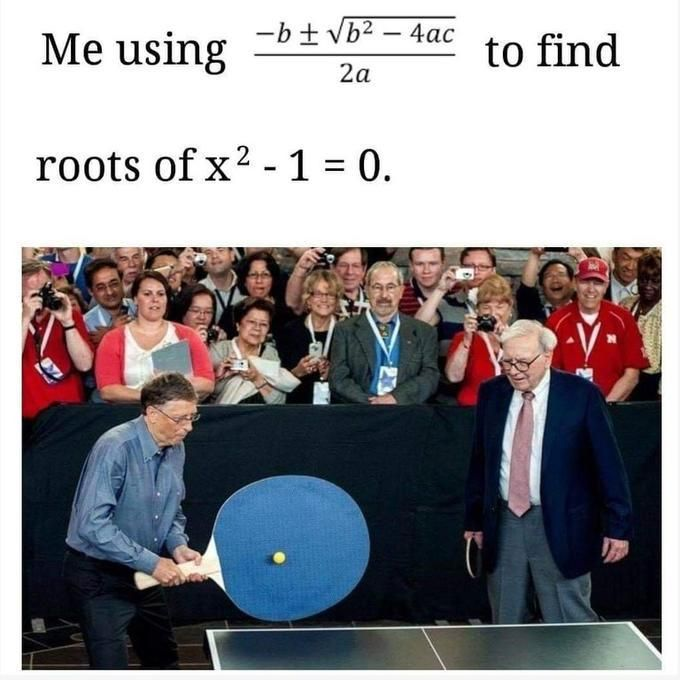
\includegraphics[width = .3\textwidth]{Figures/Histogram.jpeg}
\caption{This is Bill Gates with a giant ping pong paddle. }
\label{Bill}

\end{figure}





% New Page
\pagebreak 

Suppose you want to put two figures side by side: 

\begin{figure}[h]
\centering
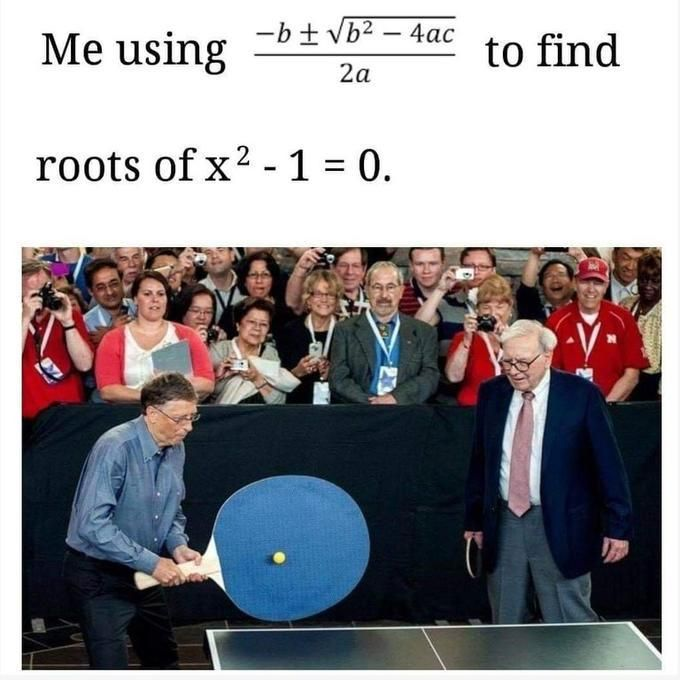
\includegraphics[width = .45\textwidth]{Figures/Histogram.jpeg}
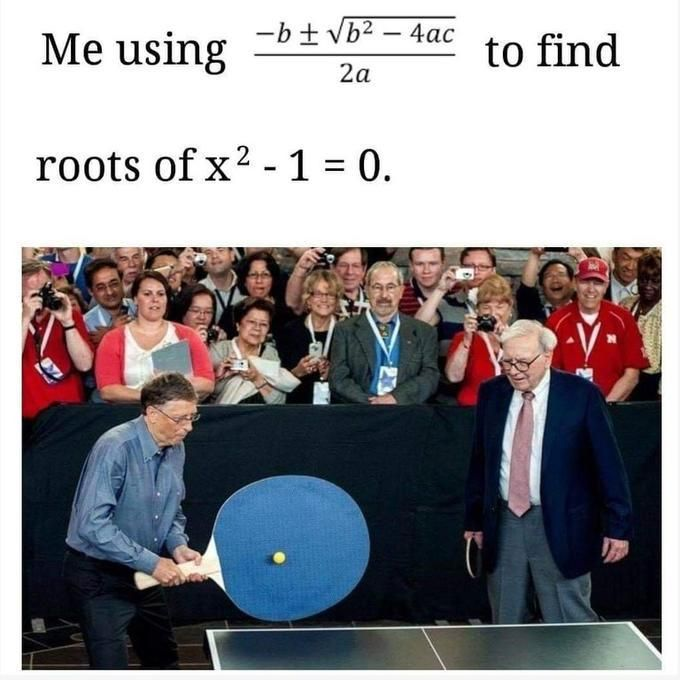
\includegraphics[width = .45\textwidth]{Figures/Histogram.jpeg}
\caption{This is Bill Gates with a giant ping pong paddle. }
\label{Bill}

\end{figure}

Remember the quadratic formula (e.g.~Figure \ref{Bill})??


% New Page
\pagebreak


\section{Tables}

This is how you insert a table: 

\begin{table}[h]
\begin{center}
\caption{ Accuracy score statistics for the random forest model.}
    \begin{tabular}[h]{ c|c|c}
    \centering
     \textbf{Statistic}& \textbf{Academic Discipline} & \textbf{Career Interests} \\
     \hline\hline
        Minimum & $0.83$ & $0.69$\\\hline
        Maximum & $0.94$ & $0.76$\\\hline
        Mean & $0.90$  & $0.71$ \\\hline
        Median & $0.92$  & $0.72$\\\hline
        Standard Deviation & $0.022$  & $0.011$\\\hline\hline
    \end{tabular}
    \label{Forest_Statistics}
\end{center}
\end{table}


\end{document}

